\chapter{Network address translation}
\label{chap:nat}

In this chapter, we're going to dig into network address translation (NAT), dynamic NAT, and port-based address translation (PAT), which is also known as NAT overload.
Of course, I'll demonstrate all the NAT commands.
I also provided some fantastic hands-on labs for you to configure at the end of this chapter, so be sure not to miss those!

It's important to understand the Cisco objectives for this chapter. They are very straightforward: you have hosts on your inside corporate
network using RFC~1918 addresses and you need to allow those hosts access to the Internet by configuring NAT translations. With that
objective in mind, that will be my direction with this chapter.

Because we'll be using ACLs in our NAT configurations, it's important
that you're really comfortable with the skills you learned in the
previous chapter before proceeding with this one.

\section{When do we use NAT?}

\emph{Network address translation} (NAT) is similar to classless inter-domain routing (CIDR) in that the original intention for NAT was to slow
the depletion of available IP address space by allowing multiple
private IP addresses to be represented by a much smaller number of public IP addresses.

Since then, it's been discovered that NAT is also a useful tool for network migrations and mergers, server load sharing, and creating
``virtual servers.''
So in this chapter, I'm going to describe the basics of NAT functionality and the terminology common to NAT.

Because NAT really decreases the overwhelming amount of public IP addresses required in a networking environment, it comes in really handy
when two companies that have duplicate internal addressing schemes merge. NAT is also a great tool to use when an organization changes its
Internet service provider (ISP) but the networking manager needs to avoid the hassle of changing the internal address scheme.

Here's a list of situations when NAT can be especially helpful:

\begin{enumerate}
   \item When you need to connect to the Internet and your hosts don't have   globally unique IP addresses
   \item When you've changed   to a new ISP that requires you to renumber your network
   \item When you need to merge two intranets with duplicate addresses
\end{enumerate}

You typically use NAT on a border router.
For example, in \vref{fig:where-configure-nat}, NAT is used on the corporate router connecting to the Internet.

\begin{figure}
   \caption{Where to configure NAT}
   \label{fig:where-configure-nat}
\end{figure}

Now you may be thinking, ``NAT's totally cool and I just gotta have it!''
But don't get too excited yet because there are some serious snags related to using NAT that you need to understand first.
Don't get me wrong -- it can truly be a lifesaver sometimes, but NAT has a bit of a dark side you need to know about too.

\paragraph{Advantages of NAT}
\begin{itemize}
   \item Conserves legally registered addresses.
   \item Remedies address overlap events.
   \item Increases flexibility when connecting to the Internet.
   \item Eliminates address renumbering as a network evolves.
\end{itemize}

\paragraph{Disadvantages of NAT}
\begin{itemize}
   \item Translation results in switching path delays.
   \item Causes loss of end-to-end IP traceability.
   \item Certain applications will not function with NAT enabled.
   \item Complicates tunneling protocols such as IPsec because NAT modifies the values in the header.
\end{itemize}


\begin{center}\rule{0.5\linewidth}{0.5pt}\end{center}

The most obvious advantage associated with NAT is that it allows you to conserve your legally registered address scheme.
But a version of it known as PAT is also why we've only just recently run out of IPv4 addresses.
Without NAT/PAT, we'd have run out of IPv4 addresses more than a decade ago!

\begin{center}\rule{0.5\linewidth}{0.5pt}\end{center}



\section{Types of network address translation}

In this section, I'm going to go over the three types of NATs with you:
\begin{description}
   \item[Static NAT (one-to-one)]
      This type of NAT is designed to allow one-to-one mapping between local and global addresses.
      Keep in mind that the static version requires you to have one real Internet IP address for every host on your network.

   \item[Dynamic NAT (many-to-one)]
      This version gives you the ability to map an unregistered IP address to a registered IP address from out of a pool of registered IP addresses.
      You don't have to statically configure your router to map each inside address to an individual outside address as you would using static NAT, but you do have to have enough real, bona fide IP addresses for everyone who's going to be sending packets to and receiving them from the Internet at the same time.

   \item[Overloading (many-to-one)]
      This is the most popular type of NAT configuration.
      Understand that overloading really is a form of dynamic NAT that maps multiple unregistered IP addresses to a single registered IP address (many-to-one) by using different source ports.
      Now, why is this so special?
      Well, because it's also known as \emph{port-based address translation} (PAT), which is also commonly referred to as NAT overload.
      Using PAT allows you to permit thousands of users to connect to the Internet using only one real global IP address -- pretty slick, right?
      Seriously, NAT overload is the real reason we haven't run out of valid IP addresses on the Internet.
      Really -- I'm not joking!
\end{description}


\begin{center}\rule{0.5\linewidth}{0.5pt}\end{center}

I'll show you how to configure all three types of NAT throughout this chapter and at the end of this chapter with the hands-on labs.

\begin{center}\rule{0.5\linewidth}{0.5pt}\end{center}



\section{NAT names}

The names we use to describe the addresses used with NAT are fairly
straightforward. Addresses used after NAT translations are called
\emph{global addresses}. These are usually the public addresses used on
the Internet, which you don't need if you aren't going on the Internet.

\emph{Local addresses} are the ones we use before NAT translation. This
means that the inside local address is actually the private address of
the sending host that's attempting to get to the Internet. The outside
local address would typically be the router interface connected to your
ISP and is also usually a public address used as the packet begins its
journey.

After translation,
the inside local address is then called the \emph{inside global address}
and the outside global address then becomes the address of the
destination host. Check out
\protect\hyperlink{c13.xhtmlux5cux23table13-2}{Table 13.2}, which lists
all this terminology and offers a clear picture of the various names
used with NAT. Keep in mind that these terms and their definitions can
vary somewhat based on implementation. The table shows how they're used
according to the Cisco exam objectives.

{\protect\hyperlink{c13.xhtmlux5cux23tableanchor13-2}{\textbf{TABLE
13.2}} NAT terms}

\begin{longtable}[]{@{}ll@{}}
\toprule
Names & Meaning\tabularnewline
\midrule
\endhead
Inside local & Source host inside address before translation -- typically
an RFC 1918 address.\tabularnewline
Outside local & Address of an outside host as it appears to the inside
network. This is usually the address of the router interface connected
to ISP -- the actual Internet address.\tabularnewline
Inside global & Source host address used after translation to get onto
the Internet. This is also the actual Internet address.\tabularnewline
Outside global & Address of outside destination host and, again, the
real Internet address.\tabularnewline
\bottomrule
\end{longtable}




\section{How NAT works}

Okay, it's time to look at how this whole NAT thing works. I'm going to
start by using \protect\hyperlink{c13.xhtmlux5cux23figure13-2}{Figure
13.2} to describe basic NAT translation.

\begin{figure}
\centering

\caption{{\protect\hyperlink{c13.xhtmlux5cux23figureanchor13-2}{\textbf{FIGURE
13.2}} Basic NAT translation}}
\end{figure}

In this figure, we
can see host 10.1.1.1 sending an Internet-bound packet to the border
router configured with NAT. The router identifies the source IP address
as an inside local IP address destined for an outside network,
translates the source IP address in the packet, and documents the
translation in the NAT table.

The packet is sent to the outside interface with the new translated
source address. The external host returns the packet to the destination
host and the NAT router translates the inside global IP address back to
the inside local IP address using the NAT table. This is as simple as it
gets!

Let's take a look at a more complex configuration using overloading,
also referred to as PAT. I'll use
\protect\hyperlink{c13.xhtmlux5cux23figure13-3}{Figure 13.3} to
demonstrate how PAT works by having an inside host HTTP to a server on
the Internet.

\begin{figure}
\centering

\caption{{\protect\hyperlink{c13.xhtmlux5cux23figureanchor13-3}{\textbf{FIGURE
13.3}} NAT overloading example (PAT)}}
\end{figure}

With PAT, all inside hosts get translated to one single IP address,
hence the term \emph{overloading}. Again, the reason we've just run out
of available global IP addresses on the Internet is because of
overloading (PAT).

Take a look at the NAT table
in\protect\hyperlink{c13.xhtmlux5cux23figure13-3}{Figure 13.3} again. In
addition to the inside local IP address and inside global IP address, we
now have port numbers. These port numbers help the router identify which
host should receive the return traffic. The router uses the source port
number from each host to differentiate the traffic from each of them.
Understand that the packet has a destination port number of 80 when it
leaves the router, and the HTTP server sends back the data with a
destination port number of 1026, in this example. This allows the NAT
translation router to differentiate between hosts in the NAT table and
then translate the destination IP address back to the inside local
address.

Port numbers are used at the Transport layer to identify the local host
in this example. If we had to use real global IP addresses to identify
the source hosts, that's called \emph{static NAT}
and we would run out
of addresses. PAT allows us to use the Transport layer to identify the
hosts, which in turn allows us to theoretically use up to about 65,000
hosts with only one real IP address!



\subsection{Static NAT configuration}

Let's take a look at a simple example of a basic static NAT
configuration:

\begin{verbatim}
ip nat inside source static 10.1.1.1 170.46.2.2
!
interface Ethernet0
 ip address 10.1.1.10 255.255.255.0
 ip nat inside
!
interface Serial0
 ip address 170.46.2.1 255.255.255.0
 ip nat outside
!
\end{verbatim}

In the preceding router output, the \texttt{ip\ nat\ inside\ source}
command identifies which IP addresses will be translated. In this
configuration example, the \texttt{ip\ nat\ inside\ source} command
configures a static translation between the inside local IP address
10.1.1.1 and the outside global IP address 170.46.2.2.

Scrolling farther down in the configuration, we find an \texttt{ip\ nat}
command under each interface. The \texttt{ip\ nat\ inside} command
identifies that interface as the inside interface. The
\texttt{ip\ nat\ outside} command identifies that interface as the
outside interface. When you look back at the
\texttt{ip\ nat\ inside\ source} command, you can see that the command
is referencing the inside interface as the source or starting point of
the translation. You could also use the command like this:
\texttt{ip\ nat\ outside\ source}. This option indicates the interface
that you designated as the outside interface should become the source or
starting point for the translation.





\subsection{Dynamic NAT configuration}

Basically, dynamic NAT really means we have a pool of addresses that
we'll use to provide real IP addresses to a group of users on the
inside. Because we don't use port numbers, we must have real IP
addresses for every user who's trying to get outside the local network
simultaneously.

Here is a sample output of a dynamic NAT configuration:

\begin{verbatim}
ip nat pool todd 170.168.2.3 170.168.2.254
netmask 255.255.255.0
ip nat inside source list 1 pool todd
!
interface Ethernet0
 ip address 10.1.1.10 255.255.255.0
 ip nat inside
!
interface Serial0
 ip address 170.168.2.1 255.255.255.0
 ip nat outside
!
access-list 1 permit 10.1.1.0 0.0.0.255
!
\end{verbatim}

The \texttt{ip\ nat\ inside\ source\ list\ 1\ pool\ todd} command tells
the router to translate IP addresses that match \texttt{access-list\ 1}
to an address found in the IP NAT pool named \texttt{todd}. Here the ACL
isn't there to filter traffic for security reasons by permitting or
denying traffic. In this case, it's there to select or designate what we
often call interesting traffic. When interesting traffic has been
matched with the access list, it's pulled into the NAT process to be
translated. This is actually a common use for access lists, which aren't
always just stuck with the dull job of just blocking traffic at an
interface!

The command
\texttt{ip\ nat\ pool\ todd\ 170.168.2.3\ 170.168.2.254\ netmask\ 255.255.255.0}
creates a pool of addresses that will be distributed to the specific
hosts that require global addresses. When troubleshooting NAT for the
Cisco objectives, always check this pool to confirm that there are
enough addresses in it to provide translation for all the inside hosts.
Last, check to make sure the pool names match exactly on both lines,
remembering that they are case sensitive; if they don't, the pool won't
work!



\subsection{PAT (overloading) configuration}

This last example shows how to configure inside global address
overloading. This is the typical form of NAT that we would use today.
It's actually now rare to use static or dynamic NAT unless it is for
something like statically mapping a server, for example.

Here is a sample output of a PAT configuration:

\begin{verbatim}
ip nat pool globalnet 170.168.2.1 170.168.2.1 netmask 255.255.255.0
ip nat inside source list 1 pool globalnet overload
!
interface Ethernet0/0
 ip address 10.1.1.10 255.255.255.0
 ip nat inside
!
interface Serial0/0
 ip address 170.168.2.1 255.255.255.0
 ip nat outside
!
access-list 1 permit 10.1.1.0 0.0.0.255
\end{verbatim}

The nice thing about
PAT is that these are only a few differences between this configuration
and the previous dynamic NAT configuration:

\begin{enumerate}
\tightlist
\item
  Our pool of addresses has shrunk to only one IP address.
\item
  We included the \texttt{overload} keyword at the end of our
  \texttt{ip\ nat\ inside\ source} command.
\end{enumerate}

A really key factor to see in the example is that the one IP address
that's in the pool for us to use is the IP address of the outside
interface. This is perfect if you are configuring NAT Overload for
yourself at home or for a small office that only has one IP address from
your ISP. You could, however, use an additional address such as
170.168.2.2 if you had that address available to you as well, and doing
that could prove very helpful in a very large implementation where
you've got such an abundance of simultaneously active internal users
that you need to have more than one overloaded IP address on the
outside!




\subsection{Simple verification of NAT}

As always, once you've chosen and configured the type of NAT you're
going to run, which is typically PAT, you must be able to verify your
configuration.

To see basic IP address translation information, use the following
command:

\begin{verbatim}
Router#show ip nat translations
\end{verbatim}

When looking at the IP NAT translations, you may see many translations
from the same host to the corresponding host at the destination.
Understand that this is typical when there are many connections to the
same server.

You can also verify your NAT configuration via the
\texttt{debug\ ip\ nat} command. This output will show the sending
address, the translation, and the destination address on each debug
line:

\begin{verbatim}
Router#debug ip nat
\end{verbatim}

But wait -- how do you clear your NAT entries from the translation table?
Just use the \texttt{clear\ ip\ nat\ translation} command, and if you
want to clear all entries from the NAT table, just use an asterisk
(\texttt{*}) at the end of the command.



\section{Testing and troubleshooting NAT}

Cisco's NAT gives you some serious power -- and it does so without much
effort, because the configurations are really pretty simple. But we all
know nothing's perfect, so in case something goes wrong, you can figure
out some of the more common culprits by running through this list of
potential causes:

\begin{enumerate}
\tightlist
\item
  Check the dynamic pools. Are they composed of the right scope of
  addresses?
\item
  Check to see if any dynamic pools overlap.
\item
  Check to see if the addresses used for static mapping and those in the
  dynamic pools overlap.
\item
  Ensure that your
  access lists specify the correct addresses for translation.
\item
  Make sure there aren't any addresses left out that need to be there,
  and ensure that none are included that shouldn't be.
\item
  Check to make sure you've got both the inside and outside interfaces
  delimited properly.
\end{enumerate}

A key thing to keep in mind is that one of the most common problems with
a new NAT configuration often isn't specific to NAT at all -- it usually
involves a routing blooper. So, because you're changing a source or
destination address in a packet, make sure your router still knows what
to do with the new address after the translation!

The first command you should typically use is the
\texttt{show\ ip\ nat\ translations} command:

\begin{verbatim}
Router#show ip nat trans
Pro   Inside global   Inside local   Outside local   Outside global
---   192.2.2.1       10.1.1.1       ---             ---
---   192.2.2.2       10.1.1.2       ---             ---
\end{verbatim}

After checking out this output, can you tell me if the configuration on
the router is static or dynamic NAT? The answer is yes, either static or
dynamic NAT is configured because there's a one-to-one translation from
the inside local to the inside global. Basically, by looking at the
output, you can't tell if it's static or dynamic per se, but you
absolutely can tell that you're not using PAT because there are no port
numbers.

Let's take a look at another output:

\begin{verbatim}
Router#sh ip nat trans
Pro Inside global      Inside local       Outside local      Outside global
tcp 170.168.2.1:11003  10.1.1.1:11003     172.40.2.2:23      172.40.2.2:23
tcp 170.168.2.1:1067   10.1.1.1:1067      172.40.2.3:23      172.40.2.3:23
\end{verbatim}

Okay, you can easily see that the previous output is using NAT Overload
(PAT). The protocol in this output is TCP, and the inside global address
is the same for both entries.

Supposedly the sky's the limit regarding the number of mappings the NAT
table can hold. But this is reality, so things like memory and CPU, or
even the boundaries set in place by the scope of available addresses or
ports, can cause limitations on the actual number of entries. Consider
that each NAT mapping devours about 160 bytes of memory. And sometimes
the amount of entries must be limited for the sake of performance or
because of policy restrictions, but this doesn't happen very often. In
situations like these, just go to the
\texttt{ip\ nat\ translation\ max-entries} command for help.

Another handy command for troubleshooting is
\texttt{show\ ip\ nat\ statistics}. Deploying this gives you a summary
of the NAT configuration, and it will count the number of active
translation types too. Also counted are hits to an existing mapping as
well any misses, with the latter causing an attempt to create a mapping.
This command will also reveal expired translations. If you want to check
into dynamic pools, their types, the total available addresses, how many
addresses have been allocated and how many have failed, plus the number
of translations that have occurred, just use the\texttt{pool} keyword
after statistics.

Here is an example of
the basic NAT debugging command:

\begin{verbatim}
Router#debug ip nat
NAT: s=10.1.1.1->192.168.2.1, d=172.16.2.2 [0]
NAT: s=172.16.2.2, d=192.168.2.1->10.1.1.1 [0]
NAT: s=10.1.1.1->192.168.2.1, d=172.16.2.2 [1]
NAT: s=10.1.1.1->192.168.2.1, d=172.16.2.2 [2]
NAT: s=10.1.1.1->192.168.2.1, d=172.16.2.2 [3]
NAT*: s=172.16.2.2, d=192.168.2.1->10.1.1.1 [1]
\end{verbatim}

Notice the last line in the output and how the \texttt{NAT} at the
beginning of the line has an asterisk (\texttt{*}). This means the
packet was translated and fast-switched to the destination. What's
fast-switched? Well in brief, fast-switching has gone by several aliases
such as cache-based switching and this nicely descriptive name, ``route
once switch many.'' The fast-switching process is used on Cisco routers
to create a cache of layer~3 routing information to be accessed at layer
2 so packets can be forwarded quickly through a router without the
routing table having to be parsed for every packet. As packets are
packet switched (looked up in the routing table), this information is
stored in the cache for later use if needed for faster routing
processing.

Let's get back to verifying NAT. Did you know you can manually clear
dynamic NAT entries from the NAT table? You can, and doing this can come
in seriously handy if you need to get rid of a specific rotten entry
without sitting around waiting for the timeout to expire! A manual clear
is also really useful when you want to clear the whole NAT table to
reconfigure a pool of addresses.

You also need to know that the Cisco IOS software just won't allow you
to change or delete an address pool if any of that pool's addresses are
mapped in the NAT table. The\texttt{clear\ ip\ nat\ translations}
command clears entries -- you can indicate a single entry via the global
and local address and through TCP and UDP translations, including ports,
or you can just type in an asterisk (\texttt{*}) to wipe out the entire
table. But know that if you do that, only dynamic entries will be
cleared because this command won't remove static entries.

Oh, and there's more -- any outside device's packet destination address
that happens to be responding to any inside device is known as the
inside global (IG) address. This means that the initial mapping has to
be held in the NAT table so that all packets arriving from a specific
connection get translated consistently. Holding entries in the NAT table
also cuts down on repeated translation operations happening each time
the same inside machine sends packets to the same outside destinations
on a regular basis.

Let me clarify: When an entry is placed into the NAT table the first
time, a timer begins ticking and its duration is known as the
translation timeout. Each time a packet for a given entry translates
through the router, the timer gets reset. If the timer expires, the
entry will be unceremoniously removed from the NAT table and the
dynamically assigned address will then be returned to the pool. Cisco's
default translation timeout is 86,400 seconds (24hours), but you can
change that with the \texttt{ip\ nat\ translation\ timeout} command.

Before we move on to the configuration section and actually use the
commands I just talked about, let's go through a couple of NAT examples
and see if you can figure out the best configuration to go with. To
start, look at \protect\hyperlink{c13.xhtmlux5cux23figure13-4}{Figure
13.4} and ask yourself two things: Where would you implement NAT in this
design? What type of NAT would you configure?



\begin{figure}
\centering

\caption{{\protect\hyperlink{c13.xhtmlux5cux23figureanchor13-4}{\textbf{FIGURE
13.4}} NAT example}}
\end{figure}

In \protect\hyperlink{c13.xhtmlux5cux23figure13-4}{Figure 13.4}, the NAT
configuration would be placed on the corporate router, just as I
demonstrated with \cref{fig:where-configure-nat}, and the configuration would be dynamic NAT with overload (PAT).
In this next NAT example, what type of NAT is being used?

\begin{verbatim}
ip nat pool todd-nat 170.168.10.10 170.168.10.20 netmask 255.255.255.0
ip nat inside source list 1 pool todd-nat
\end{verbatim}

The preceding command uses dynamic NAT without PAT. The \texttt{pool} in
the command gives the answer away as dynamic, plus there's more than one
address in the pool and there is no \texttt{overload} command at the end
of our \texttt{ip\ nat\ inside\ source} command. This means we are not
using PAT!

In the next NAT example, refer to
\protect\hyperlink{c13.xhtmlux5cux23figure13-5}{Figure 13.5} and see if
you can come up with the configuration needed.

\begin{figure}
\centering

\caption{{\protect\hyperlink{c13.xhtmlux5cux23figureanchor13-5}{\textbf{FIGURE
13.5}} Another NAT example}}
\end{figure}

\protect\hyperlink{c13.xhtmlux5cux23figure13-5}{Figure
13.5} shows a border router that needs to be configured with NAT and
allow the use of six public IP addresses to the inside locals,
192.1.2.109 through 192.1.2.114. However, on the inside network, you
have 62 hosts that use the private addresses of 192.168.10.65 through
192.168.10.126. What would your NAT configuration be on the border
router?

Actually, two different answers would both work here, but the following
would be my first choice based on the exam objectives:

\begin{verbatim}
ip nat pool Todd 192.1.2.109 192.1.2.109 netmask 255.255.255.248
access-list 1 permit 192.168.10.64 0.0.0.63
ip nat inside source list 1 pool Todd overload
\end{verbatim}

The command
\texttt{ip\ nat\ pool\ Todd\ 192.1.2.109\ 192.1.2.109\ netmask\ 255.255.255.248}
sets the pool name as Todd and creates a dynamic pool of only one
address using NAT address 192.1.2.109. Instead of the \texttt{netmask}
command, you can use the \texttt{prefix-length\ 29} statement. Just in
case you're wondering, you cannot do this on router interfaces as well!

The second answer would get you the exact same result of having only
192.1.2.109 as your inside global, but you can type this in and it will
also work:
\texttt{ip\ nat\ pool\ Todd\ 192.1.2.109\ 192.1.2.114\ netmask\ 255.255.255.248}.
But this option really is a waste because the second through sixth
addresses would only be used if there was a conflict with a TCP port
number. You would use something like what I've shown in this example if
you literally had about ten thousand hosts with one Internet connection!
You would need it to help with the TCP-Reset issue when two hosts are
trying to use the same source port number and get a negative
acknowledgment (NAK). But in our example, we've only got up to 62 hosts
connecting to the Internet at the same time, so having more than one
inside global gets us nothing!

If you're fuzzy on the second line where the access list is set in the
NAT configuration, do a quick review of Chapter 12, ``Security.'' But
this isn't difficult to grasp because it's easy to see in this
access-list line that it's just the \emph{\texttt{network\ number}} and
\emph{\texttt{wildcard}} used with that command. I always say, ``Every
question is a subnet question,'' and this one is no exception. The
inside locals in this example were 192.168.10.65--126, which is a block
of 64, or a 255.255.255.192 mask. As I've said in pretty much every
chapter, you really need to be able to subnet quickly!

The command
\texttt{ip\ nat\ inside\ source\ list\ 1\ pool\ Todd\ overload} sets the
dynamic pool to use PAT by using the \texttt{overload} command.

And be sure to add the \texttt{ip\ nat\ inside} and
\texttt{ip\ nat\ outside} statements on the appropriate interfaces.

\begin{note}
If you're planning on testing for any Cisco exam, configure the hands-on labs at the end of this chapter until you're really comfortable with doing that!
\end{note}

One more example, and then you are off to the written lab, hands-on
labs, and review questions.

The network in
\protect\hyperlink{c13.xhtmlux5cux23figure13-6}{Figure 13.6} is already
configured with IP addresses as shown in the figure, and there is only
one configured host. However, you need to add 25 more hosts to the LAN.
Now, all 26 hosts must be able to get to the Internet at the same time.

\begin{figure}
\centering
%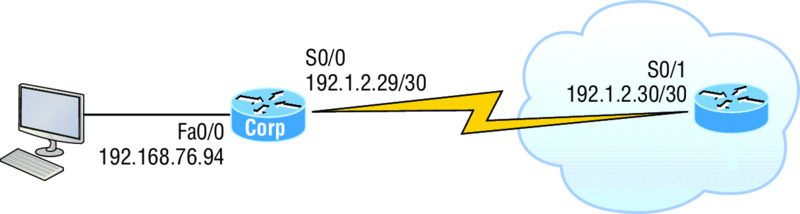
\includegraphics{images/c13f006.jpg}
\caption{{\protect\hyperlink{c13.xhtmlux5cux23figureanchor13-6}{\textbf{FIGURE
13.6}} Last NAT example}}
\end{figure}

By looking at the configured network, use only the following inside
addresses to configure NAT on the Corp router to allow all hosts to
reach the Internet:

\begin{enumerate}
\tightlist
\item
  Inside globals: 198.18.41.129 through 198.18.41.134
\item
  Inside locals: 192.168.76.65 through 192.168.76.94
\end{enumerate}

This one is a bit more challenging because all we have to help us figure
out the configuration is the inside globals and the inside locals. But
even meagerly armed with these crumbs of information, plus the IP
addresses of the router interfaces shown in the figure, we can still
configure this correctly.

To do that, we must first determine what our block sizes are so we can
get our subnet mask for our NAT pool. This will also equip us to
configure the wildcard for the access list.

You should easily be able to see that the block size of the inside
globals is 8 and the block size of the inside locals is 32. Know that
it's critical not to stumble on this foundational information!

So we can configure NAT now that we have our block sizes:

\begin{verbatim}
ip nat pool Corp 198.18.41.129 198.18.41.134 netmask 255.255.255.248
ip nat inside source list 1 pool Corp overload
access-list 1 permit 192.168.76.64 0.0.0.31
\end{verbatim}

Since we had a block of only 8 for our pool, we had to use the
\texttt{overload} command to make sure all 26 hosts can get to the
Internet at the same time.

There is one other simple way to configure NAT, and I use this command
at my home office to connect to my ISP. One command line and it's done!
Here it is:

\begin{verbatim}
ip nat inside source list 1 int s0/0/0 overload
\end{verbatim}

I can't say enough how much I love efficiency, and being able to achieve
something cool using one measly line always makes me happy! My one
little powerfully elegant line essentially says, ``Use my outside local
as my inside global and overload it.'' Nice! Of course, I still had to
create ACL 1 and add the inside and outside interface commands to the
configuration, but this is a really nice, fast way to configure NAT if
you don't have a pool of addresses to use.



\section{Summary}

Now this really was a fun chapter. Come on -- admit it! You learned a lot
about Network Address Translation (NAT) and how it's configured as
static and dynamic as well as with Port Address Translation (PAT), also
called NAT Overload.

I also described how each flavor of NAT is used in a network as well as
how each type is configured.

We finished up by going through some verification and troubleshooting
commands. Now don't forget to practice all the wonderfully helpful labs
until you've got them nailed down tight!



\section{Exam essentials}

\textbf{Understand the term \emph{NAT}.} This may come as news to you,
because I didn't -- okay, failed to -- mention it earlier, but NAT has a
few nicknames. In the industry, it's referred to as network
masquerading, IP-masquerading, and (for those who are besieged with OCD
and compelled to spell everything out) Network Address Translation.
Whatever you want to dub it, basically, they all refer to the process of
rewriting the source/destination addresses of IP packets when they go
through a router or firewall. Just focus on the process that's occurring
and your understanding of it (i.e., the important part) and you're on it
for sure!

\textbf{Remember the three methods of NAT.} The three methods are
static, dynamic, and overloading; the latter is also called PAT.

\textbf{Understand static NAT.} This type of NAT is designed to allow
one-to-one mapping between local and global addresses.

\textbf{Understand dynamic NAT.} This version gives you the ability to
map a range of unregistered IP addresses to a registered IP address from
out of a pool of registered IP addresses.

\textbf{Understand overloading.} Overloading really is a form of dynamic
NAT that maps multiple unregistered IP addresses to a single registered
IP address (many-to-one) by using different ports. It's also known as
\emph{PAT}.



\section{Written lab 13}

In this section, you'll complete the following lab to make sure you've
got the information and concepts contained within it fully dialed in:

Lab 13.1: NAT

You can find the answers to this lab in Appendix A, ``Answers to Written
Labs.''

In this section,
write the answers to the following questions:

\begin{enumerate}
\item
  What type of address translation can use only one address to allow
  thousands of hosts to be translated globally?
\item
  What command can you use to show the NAT translations as they occur on
  your router?
\item
  What command will show you the translation table?
\item
  What command will clear all your NAT entries from the translation
  table?
\item
  An inside local is before or after translation?
\item
  An inside global is before or after translation?
\item
  Which command can be used for troubleshooting and displays a summary
  of the NAT configuration as well as counts of active translation types
  and hits to an existing mapping?
\item
  What commands must be used on your router interfaces before NAT will
  translate addresses?
\item
  In the following output, what type of NAT is being used?

\begin{verbatim}
ip nat pool todd-nat 170.168.10.10 170.168.10.20 netmask 255.255.255.0
\end{verbatim}
\item
  Instead of the \texttt{netmask} command, you can use the
  \_\_\_\_\_\_\_\_\_\_\_\_\_ statement.
\end{enumerate}




\section{Hands-on labs}

I am going to use some basic routers for these labs, but really, almost
any Cisco router will work. Also, you can use the LammleSim IOS version
to run through all the labs in this (and every) chapter in this book.

Here is a list of the labs in this chapter:

\begin{enumerate}
\tightlist
\item
  Lab 13.1: Preparing for NAT
\item
  Lab 13.2: Configuring Dynamic NAT
\item
  Lab 13.3: Configuring PAT
\end{enumerate}

I am going to use the network shown in the following diagram for our
hands-on labs. I highly recommend you connect up some routers and run
through these labs. You will configure NAT on router Lab\_A to translate
the private IP address of 192.168.10.0 to a public address of
171.16.10.0.

\begin{figure}
\centering
%
\includegraphics{images/c13f007.jpg}
\caption{}
\end{figure}

\protect\hyperlink{c13.xhtmlux5cux23table13-3}{Table 13.3} shows the
commands we will use and the purpose of each command.



{\protect\hyperlink{c13.xhtmlux5cux23tableanchor13-3}{\textbf{TABLE
13.3}} Command summary for NAT/PAT hands-on labs}

\begin{longtable}[]{@{}ll@{}}
\toprule
Command & Purpose\tabularnewline
\midrule
\endhead
\texttt{ip\ nat\ inside\ source\ list}
\emph{\texttt{acl\ pool}\texttt{name}} & Translates IPs that match the
ACL to the pool\tabularnewline
\texttt{ip\ nat\ inside\ source\ static}
\emph{\texttt{inside\_addr\ outside\_addr}} & Statically maps an inside
local address to an outside global address\tabularnewline
\texttt{ip\ nat\ pool} \emph{\texttt{name}} & Creates an address
pool\tabularnewline
\texttt{ip\ nat\ inside} & Sets an interface to be an inside
interface\tabularnewline
\texttt{ip\ nat\ outside} & Sets an interface to be an outside
interface\tabularnewline
\texttt{show\ ip\ nat\ translations} & Shows current NAT
translations\tabularnewline
\bottomrule
\end{longtable}




\subsection{Lab 13.1: Preparing for NAT}

In this lab, you'll set up your routers with IP addresses and RIP
routing.

\begin{enumerate}
\item
  Configure the routers with the IP addresses listed in the following
  table:

  \begin{longtable}[]{@{}lll@{}}
  \toprule
  \textbf{Router} & \textbf{Interface} & \textbf{IP
  Address}\tabularnewline
  \midrule
  \endhead
  ISP & S0 & 171.16.10.1/24\tabularnewline
  Lab\_A & S0/2 & 171.16.10.2/24\tabularnewline
  Lab\_A & S0/0 & 192.168.20.1/24\tabularnewline
  Lab\_B & S0 & 192.168.20.2/24\tabularnewline
  Lab\_B & E0 & 192.168.30.1/24\tabularnewline
  Lab\_C & E0 & 192.168.30.2/24\tabularnewline
  \bottomrule
  \end{longtable}

  After you configure IP addresses on the routers, you should be able to
  ping from router to router, but since we do not have a routing
  protocol running until the next step, you can verify only from one
  router to another but not through the network until RIP is set up. You
  can use any routing protocol you wish; I am just using RIP for
  simplicity's sake to get this up and running.
\item
  On Lab\_A, configure RIP routing, set a passive interface, and
  configure the default network.

\begin{verbatim}
Lab_A#config t
Lab_A(config)#router rip
Lab_A(config-router)#network 192.168.20.0
Lab_A(config-router)#network 171.16.0.0
Lab_A(config-router)#passive-interface s0/2
Lab_A(config-router)#exit
Lab_A(config)#ip default-network 171.16.10.1
\end{verbatim}

  The \texttt{passive-interface} command stops RIP updates from being
  sent to the ISP and the \texttt{ip\ default-network} command
  advertises a default network to the other routers so they know how to
  get to the Internet.
\item
  On Lab\_B, configure RIP routing:

\begin{verbatim}
Lab_B#config t
Lab_B(config)#router rip
Lab_B(config-router)#network 192.168.30.0
Lab_B(config-router)#network 192.168.20.0
\end{verbatim}
\item
  On Lab\_C, configure RIP routing:

\begin{verbatim}
Lab_C#config t
Lab_C(config)#router rip
Lab_C(config-router)#network 192.168.30.0
\end{verbatim}
\item
  On the ISP router, configure a default route to the corporate network:

\begin{verbatim}
ISP#config t
ISP(config)#ip route 0.0.0.0 0.0.0.0 s0
\end{verbatim}
\item
  Configure the ISP router so you can telnet into the router without
  being prompted for a password:

\begin{verbatim}
ISP#config t
ISP(config)#line vty 0 4
ISP(config-line)#no login
\end{verbatim}
\item
  Verify that you can ping from the ISP router to the Lab\_C router and
  from the Lab\_C router to the ISP router. If you cannot, troubleshoot
  your network.
\end{enumerate}




\subsection{Lab 13.2: Configuring dynamic NAT}

In this lab, you'll configure dynamic NAT on the Lab\_A router.

\begin{enumerate}
\item
  Create a pool of addresses called GlobalNet on the Lab\_A router. The
  pool should contain a range of addresses of 171.16.10.50 through
  171.16.10.55.

\begin{verbatim}
Lab_A(config)#ip nat pool GlobalNet 171.16.10.50 171.16.10.55
net 255.255.255.0
\end{verbatim}
\item
  Create access list
  1. This list permits traffic from the 192.168.20.0 and 192.168.30.0
  network to be translated.

\begin{verbatim}
Lab_A(config)#access-list 1 permit 192.168.20.0 0.0.0.255
Lab_A(config)#access-list 1 permit 192.168.30.0 0.0.0.255
\end{verbatim}
\item
  Map the access list to the pool that was created.

\begin{verbatim}
Lab_A(config)#ip nat inside source list 1 pool GlobalNet
\end{verbatim}
\item
  Configure serial 0/0 as an inside NAT interface.

\begin{verbatim}
Lab_A(config)#int s0/0
Lab_A(config-if)#ip nat inside
\end{verbatim}
\item
  Configure serial 0/2 as an outside NAT interface.

\begin{verbatim}
Lab_A(config-if)#int s0/2
Lab_A(config-if)#ip nat outside
\end{verbatim}
\item
  Move the console connection to the Lab\_C router. Log in to the Lab\_C
  router. Telnet from the Lab\_C router to the ISP router.

\begin{verbatim}
Lab_C#telnet 171.16.10.1
\end{verbatim}
\item
  Move the console connection to the Lab\_B router. Log in to the Lab\_B
  router. Telnet from the Lab\_B router to the ISP router.

\begin{verbatim}
Lab_B#telnet 171.16.10.1
\end{verbatim}
\item
  Execute the command \texttt{show\ users} from the ISP router. (This
  shows who is accessing the VTY lines.)

\begin{verbatim}
ISP#show users
\end{verbatim}

  \begin{enumerate}
  \item
    What does it show as your source IP
    address?\_\_\_\_\_\_\_\_\_\_\_\_\_\_\_\_
  \item
    What is your real source IP
    address?\_\_\_\_\_\_\_\_\_\_\_\_\_\_\_\_\_\_

    The \texttt{show\ users} output should look something like this:

\begin{verbatim}
ISP>sh users
    Line       User       Host(s)              Idle       Location
   0 con 0                idle                 00:03:32
   2 vty 0                idle                 00:01:33 171.16.10.50
*  3 vty 1                idle                 00:00:09 171.16.10.51
  Interface  User      Mode                     Idle Peer Address
ISP>
\end{verbatim}

   \begin{note}
    Notice that there is a one-to-one translation.
    This means you must have a real IP address for every host that wants to get to the Internet, which is not typically possible.
   \end{note}
  \end{enumerate}
\item
  Leave the session open on the ISP router and connect to Lab\_A. (Use
  \textbf{Ctrl+Shift+6}, let go, and then press \textbf{X}.)
\item
  Log in to your Lab\_A router and view your current translations by
  entering the \texttt{show\ ip\ nat\ translations} command. You should
  see something like this:

\begin{verbatim}
Lab_A#sh ip nat translations
Pro Inside global      Inside local       Outside local      Outside global
--- 171.16.10.50       192.168.30.2       ---                ---
--- 171.16.10.51       192.168.20.2       ---                ---
Lab_A#
\end{verbatim}
\item
  If you turn on \texttt{debug\ ip\ nat} on the Lab\_A router and then
  ping through the router, you will see the actual NAT process take
  place, which will look something like this:

\begin{verbatim}
00:32:47: NAT*: s=192.168.30.2->171.16.10.50, d=171.16.10.1 [5]
00:32:47: NAT*: s=171.16.10.1, d=171.16.10.50->192.168.30.2
\end{verbatim}
\end{enumerate}




\subsection{Lab 13.3: Configuring PAT}

In this lab, you'll configure PAT on the Lab\_A router. We will use PAT
because we don't want a one-to-one translation, which uses just one IP
address for every user on the network.

\begin{enumerate}
\item
  On the Lab\_A router, delete the translation table and remove the
  dynamic NAT pool.

\begin{verbatim}
Lab_A#clear ip nat translations *
Lab_A#config t
Lab_A(config)#no ip nat pool GlobalNet 171.16.10.50
171.16.10.55 netmask 255.255.255.0
Lab_A(config)#no ip nat inside source list 1 pool GlobalNet
\end{verbatim}
\item
  On the Lab\_A router, create a NAT pool with one address called
  Lammle. The pool should contain a single address, 171.16.10.100. Enter
  the following command:

\begin{verbatim}
Lab_A#config t
Lab_A(config)#ip nat pool Lammle 171.16.10.100 171.16.10.100
net 255.255.255.0
\end{verbatim}
\item
  Create access list 2. It should permit networks 192.168.20.0 and
  192.168.30.0 to be translated.

\begin{verbatim}
Lab_A(config)#access-list 2 permit 192.168.20.0 0.0.0.255
Lab_A(config)#access-list 2 permit 192.168.30.0 0.0.0.255
\end{verbatim}
\item
  Map access list 2 to the new pool, allowing PAT to occur by using the
  \texttt{overload} command.

\begin{verbatim}
Lab_A(config)#ip nat inside source list 2 pool Lammle overload
\end{verbatim}
\item
  Log in to the Lab\_C router and telnet to the ISP router; also, log in
  to the Lab\_B router and telnet to the ISP router.
\item
  From the ISP router, use the \texttt{show\ users} command. The output
  should look like this:

\begin{verbatim}
ISP>sh users
    Line       User       Host(s)              Idle       Location
*  0 con 0                idle                 00:00:00
   2 vty 0                idle                 00:00:39 171.16.10.100
   4 vty 2                idle                 00:00:37 171.16.10.100
 
  Interface  User      Mode               Idle Peer Address
 
ISP>
\end{verbatim}
\item
  From the Lab\_A router, use the \texttt{show\ ip\ nat\ translations}
  command.

\begin{verbatim}
Lab_A#sh ip nat translations
Pro Inside global  Inside local  Outside local Outside global
tcp 171.16.10.100:11001 192.168.20.2:11001 171.16.10.1:23    
171.16.10.1:23
tcp 171.16.10.100:11002 192.168.30.2:11002 171.16.10.1:23    
171.16.10.1:23
\end{verbatim}
\item
  Also make sure the \texttt{debug\ ip\ nat} command is on for the
  Lab\_A router. If you ping from the Lab\_C router to the ISP router,
  the output will look like this:

\begin{verbatim}
01:12:36: NAT: s=192.168.30.2->171.16.10.100, d=171.16.10.1 [35]
01:12:36: NAT*: s=171.16.10.1, d=171.16.10.100->192.168.30.2 [35]
01:12:36: NAT*: s=192.168.30.2->171.16.10.100, d=171.16.10.1 [36]
01:12:36: NAT*: s=171.16.10.1, d=171.16.10.100->192.168.30.2 [36]
01:12:36: NAT*: s=192.168.30.2->171.16.10.100, d=171.16.10.1 [37]
01:12:36: NAT*: s=171.16.10.1, d=171.16.10.100->192.168.30.2 [37]
01:12:36: NAT*: s=192.168.30.2->171.16.10.100, d=171.16.10.1 [38]
01:12:36: NAT*: s=171.16.10.1, d=171.16.10.100->192.168.30.2 [38]
01:12:37: NAT*: s=192.168.30.2->171.16.10.100, d=171.16.10.1 [39]
01:12:37: NAT*: s=171.16.10.1, d=171.16.10.100->192.168.30.2 [39]
\end{verbatim}
\end{enumerate}



\section{Review questions}

You can find the answers to these questions in Appendix B, ``Answers to
Review Questions.''

\begin{enumerate}
\item
  Which of the following are disadvantages of using NAT? (Choose three.)

  \begin{enumerate}
  \tightlist
  \item
    Translation introduces switching path delays.
  \item
    NAT conserves legally registered addresses.
  \item
    NAT causes loss of end-to-end IP traceability.
  \item
    NAT increases flexibility when connecting to the Internet.
  \item
    Certain applications will not function with NAT enabled.
  \item
    NAT reduces address overlap occurrence.
  \end{enumerate}
\item
  Which of the following are advantages of using NAT? (Choose three.)

  \begin{enumerate}
  \tightlist
  \item
    Translation introduces switching path delays.
  \item
    NAT conserves legally registered addresses.
  \item
    NAT causes loss of end-to-end IP traceability.
  \item
    NAT increases flexibility when connecting to the Internet.
  \item
    Certain applications will not function with NAT enabled.
  \item
    NAT remedies address overlap occurrence.
  \end{enumerate}
\item
  Which command will allow you to see real-time translations on your
  router?

  \begin{enumerate}
  \tightlist
  \item
    \texttt{show\ ip\ nat\ translations}
  \item
    \texttt{show\ ip\ nat\ statistics}
  \item
    \texttt{debug\ ip\ nat}
  \item
    \texttt{clear\ ip\ nat\ translations\ *}
  \end{enumerate}
\item
  Which command will show you all the translations active on your
  router?

  \begin{enumerate}
  \tightlist
  \item
    \texttt{show\ ip\ nat\ translations}
  \item
    \texttt{show\ ip\ nat\ statistics}
  \item
    \texttt{debug\ ip\ nat}
  \item
    \texttt{clear\ ip\ nat\ translations\ *}
  \end{enumerate}
\item
  Which command will clear all the translations active on your router?

  \begin{enumerate}
  \tightlist
  \item
    \texttt{show\ ip\ nat\ translations}
  \item
    \texttt{show\ ip\ nat\ statistics}
  \item
    \texttt{debug\ ip\ nat}
  \item
    \texttt{clear\ ip\ nat\ translations\ *}
  \end{enumerate}
\item
  Which command will show you the summary of the NAT configuration?

  \begin{enumerate}
  \tightlist
  \item
    \texttt{show\ ip\ nat\ translations}
  \item
    \texttt{show\ ip\ nat\ statistics}
  \item
    \texttt{debug\ ip\ nat}
  \item
    \texttt{clear\ ip\ nat\ translations\ *}
  \end{enumerate}
\item
  Which command will create a dynamic pool named Todd that will provide
  you with 30 global addresses?

  \begin{enumerate}
  \tightlist
  \item
    \texttt{ip\ nat\ pool\ Todd\ 171.16.10.65\ 171.16.10.94\ net\ 255.255.255.240}
  \item
    \texttt{ip\ nat\ pool\ Todd\ 171.16.10.65\ 171.16.10.94\ net\ 255.255.255.224}
  \item
    \texttt{ip\ nat\ pool\ todd\ 171.16.10.65\ 171.16.10.94\ net\ 255.255.255.224}
  \item
    \texttt{ip\ nat\ pool\ Todd\ 171.16.10.1\ 171.16.10.254\ net\ 255.255.255.0}
  \end{enumerate}
\item
  Which of the following are methods of NAT? (Choose three.)

  \begin{enumerate}
  \tightlist
  \item
    Static
  \item
    IP NAT pool
  \item
    Dynamic
  \item
    NAT double-translation
  \item
    Overload
  \end{enumerate}
\item
  When creating a pool of global addresses, which of the following can
  be used instead of the \texttt{netmask} command?

  \begin{enumerate}
  \tightlist
  \item
    \texttt{/} (slash notation)
  \item
    \texttt{prefix-length}
  \item
    \texttt{no\ mask}
  \item
    \texttt{block-size}
  \end{enumerate}
\item
  Which of the following would be a good starting point for
  troubleshooting if your router is not translating?

  \begin{enumerate}
  \tightlist
  \item
    Reboot.
  \item
    Call Cisco.
  \item
    Check your interfaces for the correct configuration.
  \item
    Run the \texttt{debug\ all} command.
  \end{enumerate}
\item
  Which of the following would be good reasons to run NAT? (Choose
  three.)

  \begin{enumerate}
  \tightlist
  \item
    You need to connect to the Internet and your hosts don't have
    globally unique IP addresses.
  \item
    You change to a new ISP that requires you to renumber your network.
  \item
    You don't want any hosts connecting to the Internet.
  \item
    You require two intranets with duplicate addresses to merge.
  \end{enumerate}
\item
  Which of the
  following is considered to be the inside host's address after
  translation?

  \begin{enumerate}
  \tightlist
  \item
    Inside local
  \item
    Outside local
  \item
    Inside global
  \item
    Outside global
  \end{enumerate}
\item
  Which of the following is considered to be the inside host's address
  before translation?

  \begin{enumerate}
  \tightlist
  \item
    Inside local
  \item
    Outside local
  \item
    Inside global
  \item
    Outside global
  \end{enumerate}
\item
  By looking at the following output, determine which of the following
  commands would allow dynamic translations?

\begin{verbatim}
Router#show ip nat trans
Pro   Inside global   Inside local   Outside local Outside global
---   1.1.128.1       10.1.1.1       ---           ---
---   1.1.130.178     10.1.1.2       ---           ---
---   1.1.129.174     10.1.1.10      ---           ---
---   1.1.130.101     10.1.1.89      ---           ---
---   1.1.134.169     10.1.1.100     ---           ---
---   1.1.135.174     10.1.1.200      ---           ---
\end{verbatim}

  \begin{enumerate}
  \tightlist
  \item
    \texttt{ip\ nat\ inside\ source\ pool\ todd\ 1.1.128.1\ 1.1.135.254\ prefix-length\ 19}
  \item
    \texttt{ip\ nat\ pool\ todd\ 1.1.128.1\ 1.1.135.254\ prefix-length\ 19}
  \item
    \texttt{ip\ nat\ pool\ todd\ 1.1.128.1\ 1.1.135.254\ prefix-length\ 18}
  \item
    \texttt{ip\ nat\ pool\ todd\ 1.1.128.1\ 1.1.135.254\ prefix-length\ 21}
  \end{enumerate}
\item
  Your inside locals are not being translated to the inside global
  addresses. Which of the following commands will show you if your
  inside globals are allowed to use the NAT pool?

\begin{verbatim}
ip nat pool Corp 198.18.41.129 198.18.41.134 netmask 255.255.255.248
ip nat inside source list 100 int s0/0 Corp overload
\end{verbatim}

  \begin{enumerate}
  \tightlist
  \item
    \texttt{debug\ ip\ nat}
  \item
    \texttt{show\ access-list}
  \item
    \texttt{show\ ip\ nat\ translation}
  \item
    \texttt{show\ ip\ nat\ statistics}
  \end{enumerate}
\item
  Which command would
  you place on the interface of a private network?

  \begin{enumerate}
  \tightlist
  \item
    \texttt{ip\ nat\ inside}
  \item
    \texttt{ip\ nat\ outside}
  \item
    \texttt{ip\ outside\ global}
  \item
    \texttt{ip\ inside\ local}
  \end{enumerate}
\item
  Which command would you place on an interface connected to the
  Internet?

  \begin{enumerate}
  \tightlist
  \item
    \texttt{ip\ nat\ inside}
  \item
    \texttt{ip\ nat\ outside}
  \item
    \texttt{ip\ outside\ global}
  \item
    \texttt{ip\ inside\ local}
  \end{enumerate}
\item
  Port Address Translation is also called what?

  \begin{enumerate}
  \tightlist
  \item
    NAT Fast
  \item
    NAT Static
  \item
    NAT Overload
  \item
    Overloading Static
  \end{enumerate}
\item
  What does the asterisk (*) represent in the following output?

\begin{verbatim}
NAT*: s=172.16.2.2, d=192.168.2.1->10.1.1.1 [1]
\end{verbatim}

  \begin{enumerate}
  \tightlist
  \item
    The packet was destined for a local interface on the router.
  \item
    The packet was translated and fast-switched to the destination.
  \item
    The packet attempted to be translated but failed.
  \item
    The packet was translated but there was no response from the remote
    host.
  \end{enumerate}
\item
  Which of the following needs to be added to the configuration to
  enable PAT?

\begin{verbatim}
ip nat pool Corp 198.18.41.129 198.18.41.134 netmask 255.255.255.248
access-list 1 permit 192.168.76.64 0.0.0.31
\end{verbatim}

  \begin{enumerate}
  \tightlist
  \item
    \texttt{ip\ nat\ pool\ inside\ overload}
  \item
    \texttt{ip\ nat\ inside\ source\ list\ 1\ pool\ Corp\ overload}
  \item
    \texttt{ip\ nat\ pool\ outside\ overload}
  \item
    \texttt{ip\ nat\ pool\ Corp\ 198.41.129\ net\ 255.255.255.0\ overload}
  \end{enumerate}
\end{enumerate}

